% --------------------------------------------------------------
% This is all preamble stuff that you don't have to worry about.
% Head down to where it says "Start here"
% --------------------------------------------------------------
 
\documentclass[12pt]{article}
 
\usepackage[margin=1in]{geometry} 
\usepackage{setspace,fancyhdr,listings,xcolor,graphicx}
\lstset{
    language=C,
    numbers=left,
    numberstyle=\tiny\color{gray},
    stepnumber=1,
    numbersep=10pt,
    backgroundcolor=\color{white},
    showspaces=false,
    showstringspaces=false,
    showtabs=false,
    frame=single,
    rulecolor=\color{black},
    tabsize=2,
    captionpos=b,
    breaklines=true,
    breakatwhitespace=false,
    title=\lstname,
    keywordstyle=\color{blue},
    commentstyle=\color{green},
    stringstyle=\color{red},
    basicstyle=\ttfamily\footnotesize,
    escapeinside={\%*}{*)},
    morekeywords={*,...},
    lineskip=-1pt % Adjust this value to make lines more compact
}
\pagestyle{fancy}
\fancyhf{}

\setlength{\headheight}{15pt}
\fancyhead[R]{Topete \thepage}

\begin{document}
 
% --------------------------------------------------------------
%                         Start here
% --------------------------------------------------------------
 
\title{EC 1: HGK}
\author{Danny Topete\\ %replace with your name
EE/CS 120B}

\maketitle

\doublespacing

% TODO Make sure to fix this bad boy up
For my real-world embedded system, I will make an automated hydroponic controller.
I call it the Hydroponic Garten Kontroller \textbf{(HGK)}. 
The world of hydroponics is a fascinating one,
Hydroponics is a method of growing plants without soil,
using mineral nutrient solutions in a water solvent.
It is interesting because every part of it is artificial to make
the plant grow in an optimally controlled environment. 
Plus you can grow plants indoors, year round without the use of pesticides.

This system will have sensors for water level, nutrient level, light, and temperature.
All important factors for growing plants. To accompany the sensors, there will be pumps for water and nutrients,
along with a grow light and a heater/cooler. 
\pagebreak
\section{Inputs:}

\begin{tabular}{ l l l }
   \textbf{A0}: & Water Level Sensor & \quad (0 = Low; 1 = Normal) \\
   \textbf{A1}: & Nutrient Level Sensor & \quad (0 = Low; 1 = Normal) \\
   \textbf{A2}: & Light Sensor & \quad (0 = Low; 1 = Normal) \\
   \textbf{A3}: & Temperature Sensor & \quad (0 = Out Of Range; 1 = Normal) \\
   \textbf{A4}: & Manual Override Switch & \quad (0 = Auto; 1 = Manual) \\
   \textbf{A5}: & Emergency Stop Button & \quad (0 = Running; 1 = Stop) \\
   \textbf{A6}: & Timer Signal & \quad (Scheduled watering and light) \\
   \textbf{A7}: & Reset Signal & \quad (0 = Normal; 1 = Reset) \\
\end{tabular}

\section{Outputs:}

\begin{tabular}{ l l l }

   \textbf{B0}: & Water Pump & \quad (0 = Off; 1 = On) \\
   \textbf{B1}: & Nutrient Pump & \quad (0 = Off; 1 = On) \\
   \textbf{B2}: & Grow Light & \quad (0 = Off; 1 = On) \\
   \textbf{B3}: & Heater/Cooler & \quad (0 = Off; 1 = On) \\
   \textbf{B4}: & Status LED & \quad (0 = Off; 1 = On) \\
   \textbf{B5}: & Alarm & \quad (0 = Off; 1 = On) \\
   \textbf{B6}: & Manual Override Signal & \quad (0 = Off; 1 = On) \\
   \textbf{B7}: & System Status & \quad (0 = Off; 1 = On) \\
\end{tabular}

\pagebreak
\section{States:}

\begin{enumerate}
  \item\textbf{INIT:}\\
    State initializes all sensors and outputs to default values.
    It goes back to this state after the Reset signal \textbf{(A7)} is received.
  \item\textbf{Idle State:}\\
    Monitors inputs without making any changes. Transitions to the necessary states based on the inputs.
  \item\textbf{Watering State:}\\
    Activates water pumps based on Water Level Sensor \textbf{(A0)}.
  \item\textbf{Nutrient State:}\\
    Activates the nutrient pump based on Nutrient Level Sensor \textbf{(A1)}.
  \item\textbf{Lighting Kontrol State:}\\
    Activates based on Light Sensor \textbf{(A2)}.
  \item\textbf{Temperature Kontrol State:}\\
    Activates based on Temperature Sensor \textbf{(A3)}.
  \item\textbf{Manual Override State:}\\
    Activates based on Manual Override Switch \textbf{(A4)}.
  \item\textbf{Stop State:}\\
  The Stop State turns off all outputs. It is an Emergency Shutoff, given the sensors have strange readings or manual intervention.
  This could be if a sensor is giving out a strange reading; which could be a sign of a malfunction or physical damage.
    It should be able to send out a mass email and SMS to everyone with a log file attached.
\end{enumerate}

\pagebreak
\section{State Transitions:}

\begin{itemize}
  \item if \textbf{(A0)}, transition to Watering State.
    Until the Water Level Sensor \textbf{(A0)} is normal, the system will stay in the Watering State.
  \item if \textbf{(A1)}, transition to Nutrient State.
    Until the Nutrient Level Sensor \textbf{(A1)} is normal, the system will stay in the Nutrient State.
  \item if \textbf{(A2)}, transition to Lighting Kontrol State.
    Until the Light Sensor \textbf{(A2)} is normal, the system will stay in the Lighting Kontrol State.
  \item if \textbf{(A3)}, transition to Temperature.
    Until the Temperature Sensor \textbf{(A3)} is normal, the system will stay in the Temperature.
  \item if \textbf{(A4)}, transition to Manual Override State.
    Until the Manual Override Switch \textbf{(A4)} is normal, the system will stay in the Manual Override
  \item if \textbf{(A5)}, transition to Stop State.
    Until the Emergency Stop Button \textbf{(A5)} is normal, the system will stay in the Stop State.
  \item if \textbf{(A6)}, transition to Timer State to do regular maintenance, such as lighting and watering.
    This would probably be its own state machine that affects A0, A1, A2, B0, B1, and B2 based upon a schedule.
  \item if \textbf{(A7)}, transition to INIT State.
    Until the Reset Signal \textbf{(A7)} is normal, the system will stay in the INIT State.
\end{itemize} 
 
\pagebreak
\section{SM Chart:}

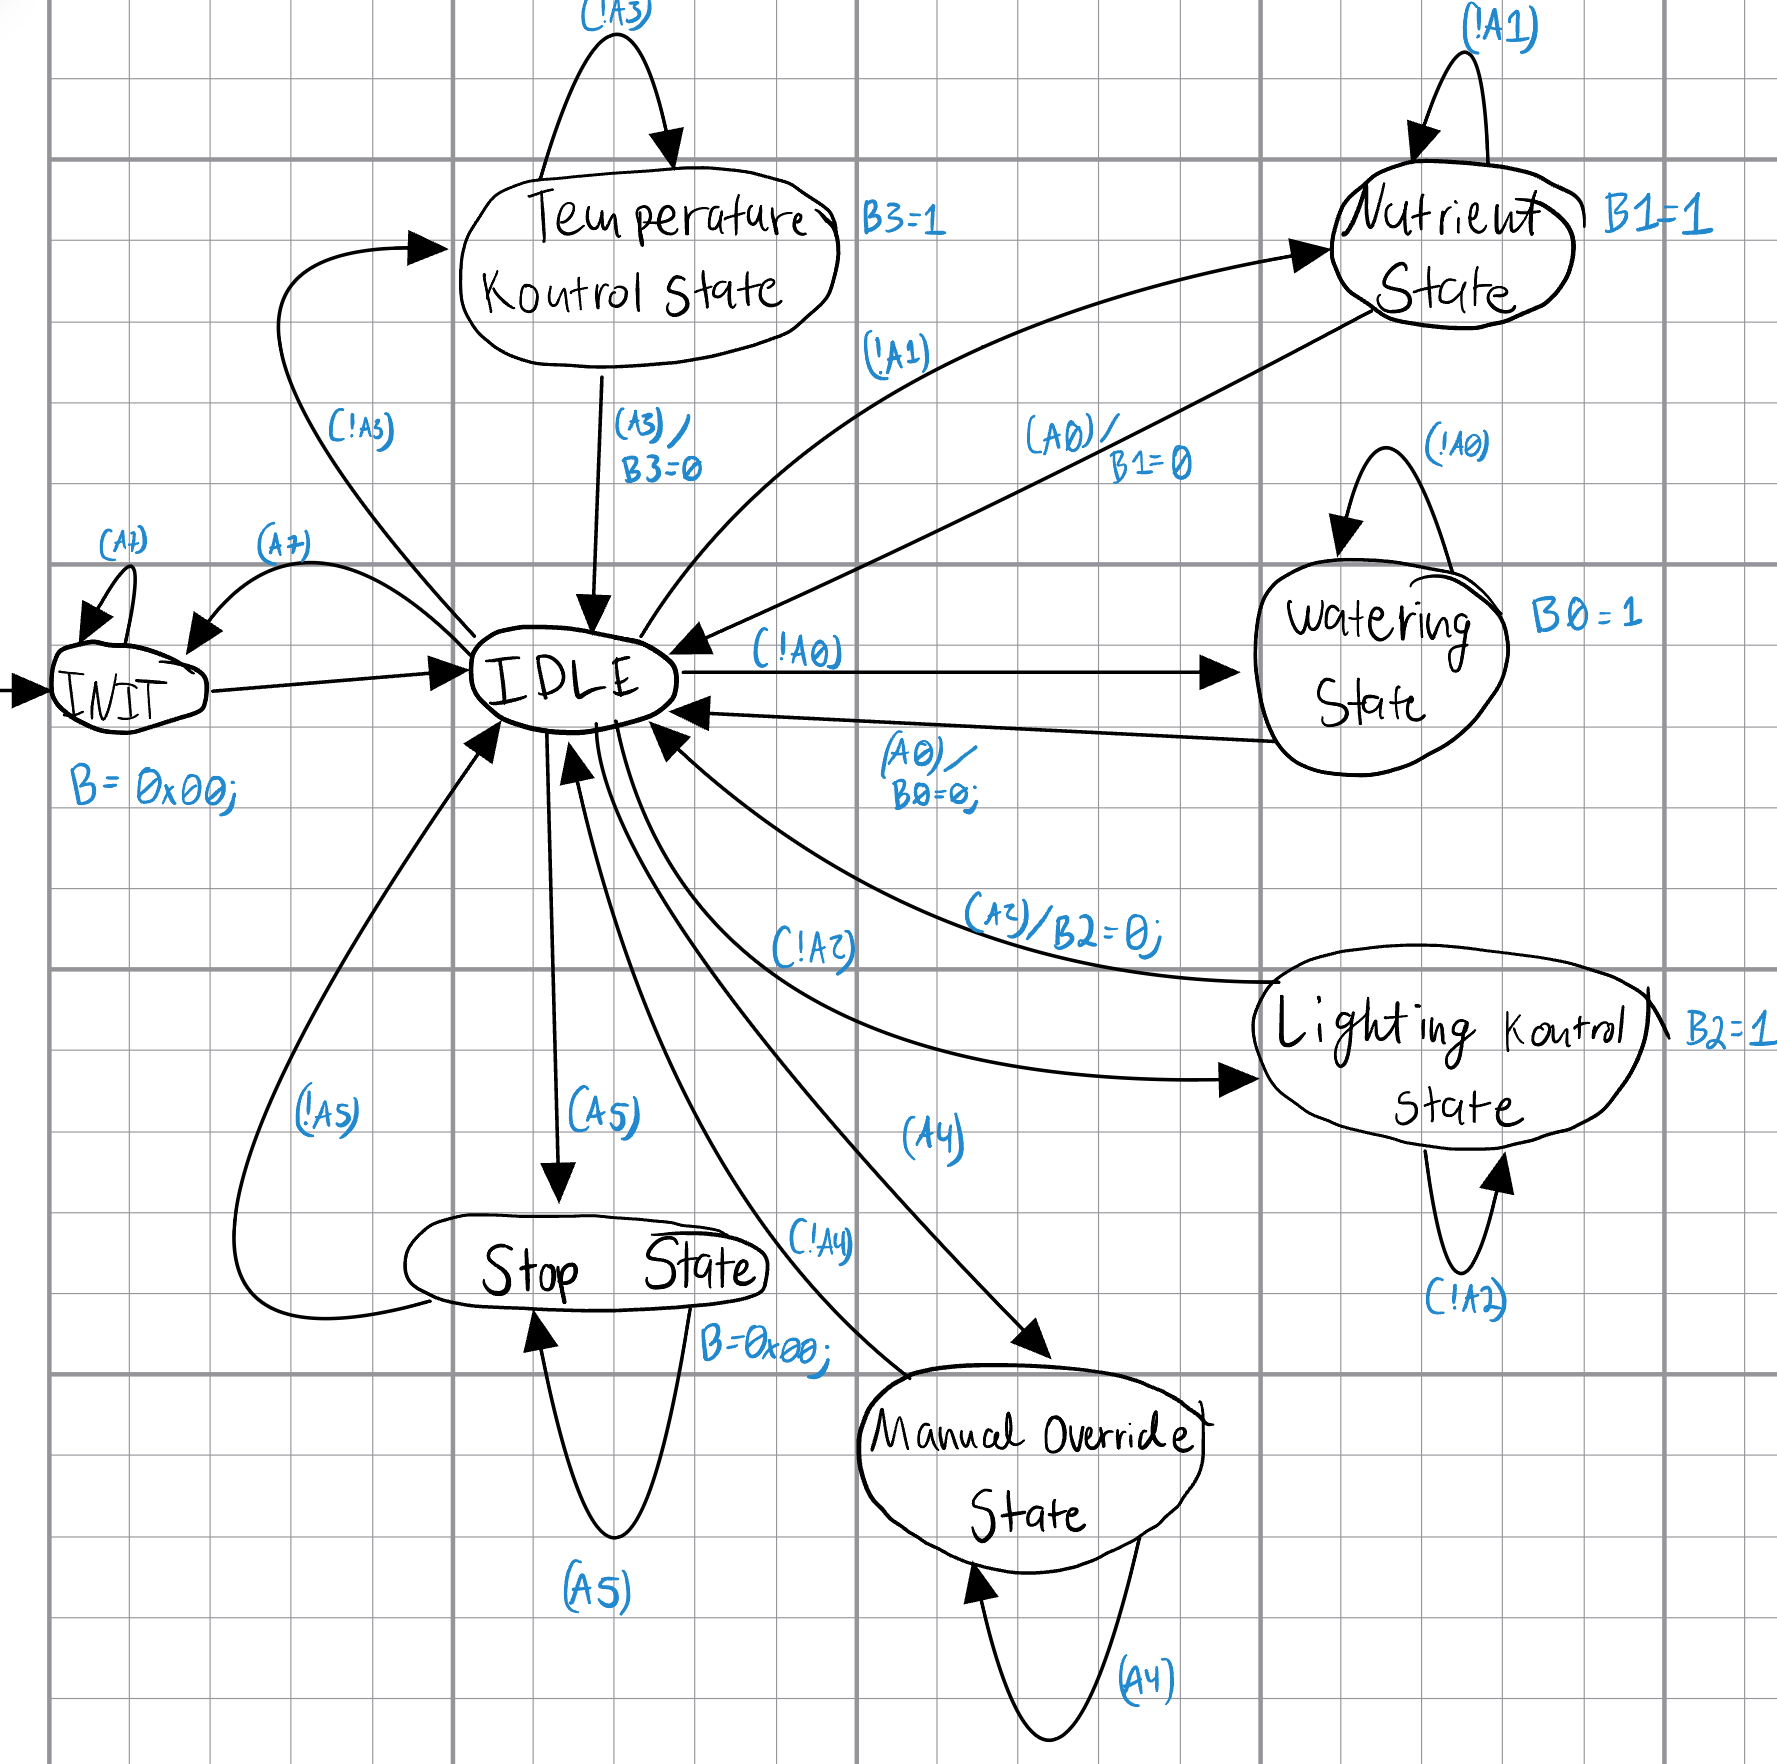
\includegraphics[width=\textwidth]{120B-EC1.jpeg.png}

  I am aware that I excluded A6, the Timer State.
  That is due to the limitation that it would probably be its own state machine to have the desired behavior.
  I am also aware with the lack of concurrency in the state machine.
  \pagebreak

  \section{SM in RIMS}
  \begin{lstlisting}[language=C]
#include "rims.h"

enum states {
  INIT,
  IDLE,
  WATERING,
  NUTRIENT,
  LIGHTING_KONTROL,
  TEMPERATURE_KONTROL,
  MANUAL_OVERRIDE,
  STOP
} State;

// State machine function
void Tick() {
  // State Transitions
  switch (State) {
  case INIT:
    // Initialize all sensors and outputs to default values
    if (A & 0x40) {
      State = INIT;
    }
    State = IDLE;

  case IDLE:
    if (~A & 0x01)
      State = WATERING;
    if (~A & 0x02)
      State = NUTRIENT;
    if (~A & 0x04)
      State = LIGHTING_KONTROL;
    if (~A & 0x08)
      State = TEMPERATURE_KONTROL;
    if (A & 0x10)
      State = MANUAL_OVERRIDE;
    if (A & 0x20)
      State = STOP;
    if (A & 0x40)
      State = INIT;
    State = IDLE;
    break;

  case WATERING:
    if (A & 0x01) {
      B = B & ~0x01;
      State = IDLE;
    }
    State = WATERING;
    break;

  case NUTRIENT:
    if (A & 0x02) {
      B = B & ~0x02;
      State = IDLE;
    }
    State = NUTRIENT;
    break;

  case LIGHTING_KONTROL:
    if (A & 0x04) {
      B = B & ~0x04;
      State = IDLE;
    }
    State = LIGHTING_KONTROL;
    break;

  case TEMPERATURE_KONTROL:
    if (A & 0x08) {
      B = B & ~0x08;
      State = IDLE;
    }
    State = TEMPERATURE_KONTROL;
    break;

  case MANUAL_OVERRIDE:
    if (~A & 0x10) {
      State = IDLE;
    }
    State = MANUAL_OVERRIDE;
    break;

  case STOP:
    if (~A & 0x20) {
      State = IDLE;
    }
    State = STOP;
    break;

  default:
    State = INIT;
    break;
  }

  // State Actions
  switch (State) {
  case INIT:
    B = 0x00;
    break;

  case IDLE:
    break;

  case WATERING:
    // B0 = 1;
    B = B | 0x01;
    break;

  case NUTRIENT:
    // B1 = 1;
    B = B | 0x02;
    break;

  case LIGHTING_KONTROL:
    // B2 = 1;
    B = B | 0x04;
    break;

  case TEMPERATURE_KONTROL:
    // B3 = 1;
    B = B | 0x08;
    break;

  case MANUAL_OVERRIDE:
    break;

  case STOP:
    B = 0x00;
    break;

  case default:
    break;
  }
}

int main() {

  State = INIT;

  while (1) {
    Tick();
  }

  return 0;
}

  \end{lstlisting}
% --------------------------------------------------------------
%     You don't have to mess with anything below this line.
% --------------------------------------------------------------
 
\end{document}t
